\documentclass[12pt,a4paper]{article}
\usepackage[spanish]{babel}
\usepackage[utf8]{inputenc}
\usepackage[T1]{fontenc}
\usepackage{geometry}
\geometry{margin=2.4cm}
\usepackage{graphicx}
\usepackage{setspace}
\usepackage{booktabs}
\usepackage{tabularx}
\usepackage{caption}
\usepackage{hyperref}
\hypersetup{colorlinks=true,linkcolor=black,urlcolor=blue,citecolor=black}
\setstretch{1.15}
\graphicspath{{figuras/}}
\captionsetup{font=small,skip=4pt}

\title{\textbf{Informe de diseño de pantallas y del flujo principal}\\[0.4em]
\large PetCare: identificación y cuidado de perros y gatos mediante un llavero NFC}
\author{Evelyn Valverde\\Aidan Carpio\\Sebastián Chocho}
\date{Loja, 23 de noviembre de 2026}

\begin{document}

\begin{center}
{\large UNIVERSIDAD INTERNACIONAL DEL ECUADOR}\\[0.2em]
Facultad de Ciencias Técnicas\\
Ingeniería en Tecnologías de la Información\\[0.8em]
{\large \textbf{Interacción Hombre-Computadora}}
\end{center}

\maketitle
\thispagestyle{empty}
\newpage

\section{Introducción}

PetCare es una aplicación web para que la dueña de un perro o un gato reconozca a su mascota y, si el animal se pierde, permita que otra persona la identifique al acercar el celular al llavero NFC del collar. El problema de interacción no es técnico: quien encuentra a un animal en la calle no va a crear una cuenta, y la dueña no debería publicar en ese llavero las vacunas, la dirección ni toda su agenda veterinaria.

Este informe describe el diseño de las pantallas y el recorrido principal de esa tarea. El producto ya no es solo una maqueta visual. El panel, las cuentas, las mascotas, los cuidados, los llaveros y los avisos de quien encuentra al animal se guardan en un servidor local del mismo proyecto. La interfaz se recorrió con la cuenta de ejemplo de Evelyn y con su perro Max, un golden retriever de 3 años y 28,4~kg, atendido en la Clínica Pañas.

El trabajo se sitúa en el diseño centrado en las personas. La norma ISO~9241-210 plantea entender el contexto de uso, especificar requisitos, producir soluciones y evaluarlas. Aquí el contexto tiene dos momentos distintos: el de la dueña, que entra con calma a revisar a su mascota, y el de quien escanea el collar, que necesita un dato útil en pocos segundos y sin registrarse.

\section{Objetivo}

Diseñar y dejar recorrido el flujo con el que la dueña inicia sesión, ve a su mascota, reporta un extravío y permite que otra persona abra el perfil público del llavero sin tener cuenta. Cada pantalla debe dejar clara una sola acción y debe usar el mismo lenguaje visual, para que el paso de una a otra no parezca un producto distinto.

El objetivo de interacción se cumple cuando ocurren tres cosas, en este orden. Primero, la dueña reconoce a su mascota en el panel sin buscar entre menús. Segundo, puede marcarla como extraviada y esa condición se ve en el perfil público. Tercero, una persona sin cuenta abre ese perfil, ve el contacto que la dueña autorizó y puede dejarle un aviso.

\section{Usuarios}

La persona principal es la dueña de la mascota. En la cuenta de ejemplo es Evelyn Valverde, de Loja. Usa el celular o el computador para saber si el llavero sigue activo, cuál es la próxima cita y qué hacer si Max no aparece. No se asume que conozca qué es un identificador NFC. Por eso el código se muestra como un llavero, con un verbo concreto: desactivar, simular escaneo o ver el perfil público.

La segunda persona es quien encuentra al animal. No tiene cuenta, no conoce a la dueña y puede estar en la calle. Su pantalla no pide registro. Muestra el nombre, la especie, la edad, la foto y, solo si la dueña lo permitió, el celular y un formulario corto. Las vacunas, las citas y la dirección no salen en ese perfil, aunque existan en el panel.

Esa separación evita mezclar dos tareas con ritmos distintos. La dueña puede detenerse a leer la agenda. Quien escanea el collar necesita una respuesta inmediata. Norman describe este ajuste como reducir la distancia entre lo que la persona quiere hacer y lo que el sistema le deja hacer. En PetCare, escanear no abre el panel privado: abre solo lo que sirve para devolver a la mascota.

\section{Decisiones de la interfaz}

El acceso y el panel comparten la misma paleta. El verde profundo del formulario de inicio de sesión es el de la barra lateral, y el verde menta del botón \emph{Entrar al panel} es el del ítem activo del menú. Así, después de entrar, la persona reconoce que sigue en el mismo producto. El fondo del panel es claro, para que las tarjetas blancas de la mascota y de los cuidados se lean como objetos separados.

Cada pantalla nombra una tarea. Inicio resume a la mascota elegida. Mis mascotas administra fichas. Cuidados guarda la agenda privada. Llaveros NFC controla el código del collar. Ajustes decide qué se publica. No se acumulan esas tareas en una sola vista, porque una pantalla cargada obliga a recordar dónde estaba cada acción. Krug recomienda quitar lo que no ayuda a decidir el siguiente paso. Esa idea guía el perfil público: no hay menú del panel ni datos clínicos.

Los estados se dicen con palabras, no solo con color. \emph{A salvo} y \emph{Extraviado}, \emph{Activo} e \emph{Inactivo}, y los avisos de guardado aparecen en texto. El color refuerza el mensaje, pero no es el único canal. El botón de reportar extravío usa un tono de alerta, distinto del verde de las acciones habituales, para que no se pulse por costumbre.

\section{Flujo principal}

El recorrido está ordenado según la tarea, no según el menú. La dueña entra, reconoce a su mascota y, si hace falta, cambia su estado. Quien encuentra al animal llega al mismo perfil por el llavero, sin pasar por el inicio de sesión.

\begin{table}[ht]
\centering
\small
\begin{tabularx}{\textwidth}{c l X}
\toprule
\textbf{Orden} & \textbf{Pantalla} & \textbf{Acción de la persona} \\
\midrule
1 & Iniciar sesión & Entra con su correo o usa la cuenta de ejemplo. \\
2 & Crear cuenta & Si no tiene cuenta, registra nombre, celular y contraseña. \\
3 & Inicio & Ve la mascota, el peso, la próxima cita y el llavero. \\
4 & Mis mascotas & Consulta la ficha o registra otra, con hasta tres fotos. \\
5 & Cuidados & Revisa vacunas, citas y desparasitación. Esos datos no se publican. \\
6 & Llaveros NFC & Simula el escaneo o desactiva el código del collar. \\
7 & Perfil público & Quien encuentra al animal abre el perfil sin cuenta. \\
8 & Aviso & Deja su nombre y un mensaje. Llega a la campana del panel. \\
9 & Extravío & La dueña marca perdida o encontrada. El perfil cambia el aviso. \\
10 & Ajustes & Decide si el celular y el formulario se muestran al escanear. \\
\bottomrule
\end{tabularx}
\caption{Orden del flujo principal de PetCare.}
\end{table}

La cuenta de ejemplo permite repetir el recorrido sin crear datos nuevos. El correo es \texttt{evelyn@petcare.ec} y la contraseña es \texttt{Petcare2026}. El botón \emph{Usar la cuenta de ejemplo} escribe esos datos en el formulario. El llavero de Max es \texttt{NFC-7F3A9C2E18B4} y su perfil público se abre en la ruta \texttt{/perfil/max}.

\section{Pantallas}

\subsection{Iniciar sesión}

La pantalla ocupa toda la ventana. A la izquierda está la ilustración del perro y el gato; a la derecha, el formulario sobre el verde del producto. No hay un marco alrededor de la tarjeta. El logo queda sobre la ilustración y el formulario concentra correo, contraseña, recordarme, recuperar la clave y crear cuenta.

Recordarme guarda la sesión en el navegador. Si no se marca, la sesión dura solo mientras la pestaña sigue abierta. \emph{Olvidé mi contraseña} lleva a un paso aparte. El texto de ayuda al pie muestra la cuenta de ejemplo, y el botón la coloca en los campos.

\begin{figure}[ht]
\centering
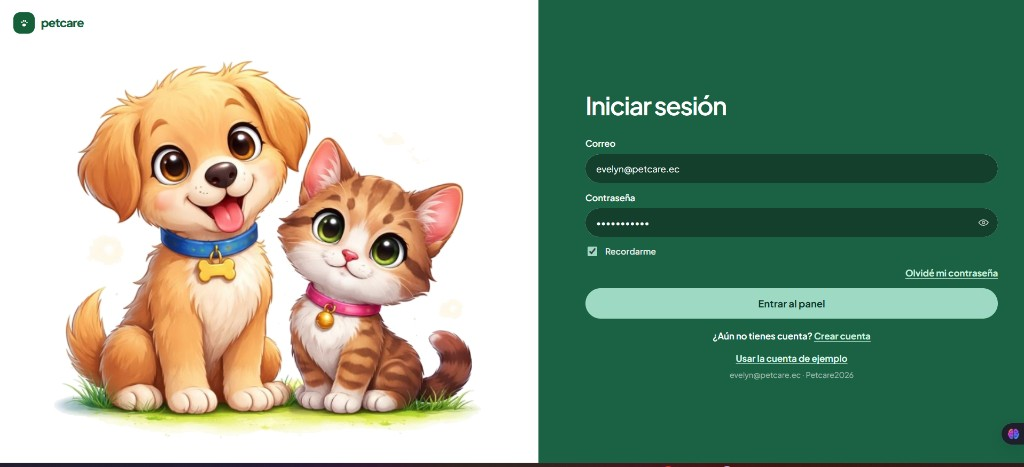
\includegraphics[width=0.92\textwidth]{01-login.png}
\caption{Inicio de sesión. La ilustración y el formulario comparten la ventana, sin marco exterior.}
\end{figure}

\subsection{Crear cuenta}

El registro pide solo lo que el producto usa después: nombre, correo, celular y contraseña. El celular se explica en el propio campo: servirá como contacto si la dueña autoriza mostrarlo en el perfil público. La contraseña pide un mínimo de ocho caracteres, letras y al menos un número, y hay que repetirla. Antes de crear la cuenta, la persona marca que entiende qué datos pueden aparecer al escanear el llavero.

Una cuenta nueva entra a un panel vacío. No hereda a Max ni sus cuidados. Así se distingue la demostración de un uso real: cada dueña arma su propia ficha.

\begin{figure}[ht]
\centering
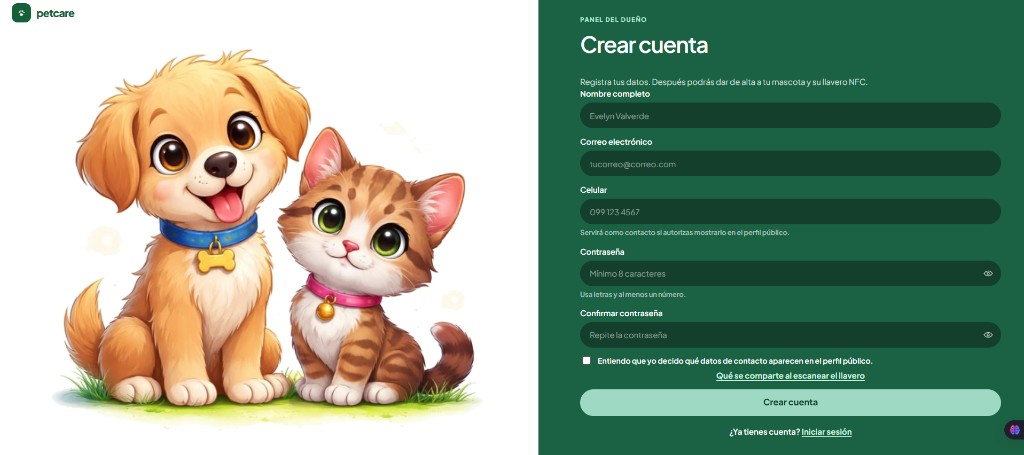
\includegraphics[width=0.92\textwidth]{02-registro.png}
\caption{Crear cuenta. El celular se explica como dato del perfil público.}
\end{figure}

\subsection{Inicio}

Después de entrar, el saludo usa el nombre de la cuenta y el resumen nombra a la mascota elegida. En la demostración se lee \emph{Buenas noches, Evelyn} y el resumen de Max. La tarjeta junta la foto, la raza, la edad, el peso, la próxima cita y el estado del llavero. Las dos acciones de esta pantalla son \emph{Ver perfil público} y \emph{Reportar como extraviado}. La agenda muestra la vacuna antirrábica del 18 de noviembre en la Clínica Pañas, el control del 24 de noviembre con la Dra.~Violeta Torres y la desparasitación del 2 de diciembre.

El menú lateral permanece visible en el computador. El ítem activo se pinta de menta, el mismo tono del botón principal del acceso.

\begin{figure}[ht]
\centering
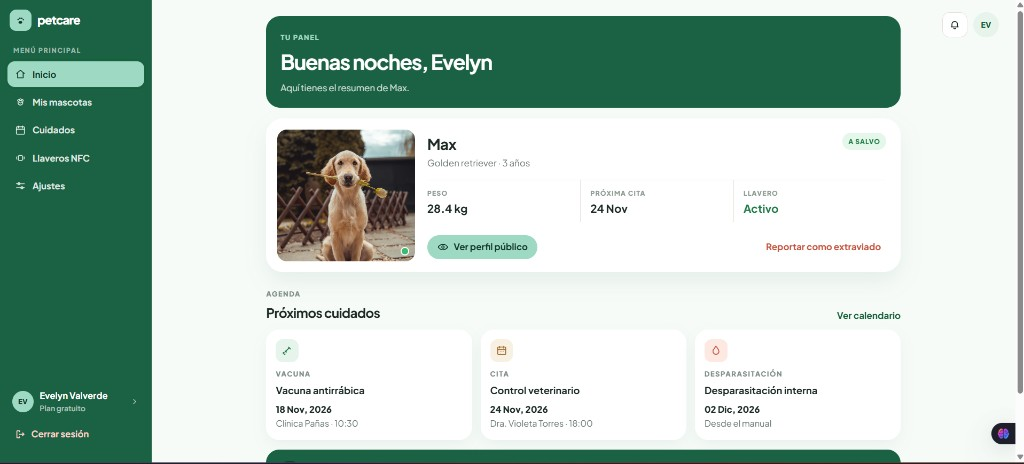
\includegraphics[width=0.92\textwidth]{03-inicio.png}
\caption{Inicio. La tarjeta de Max reúne identidad, peso, próxima cita y estado del llavero.}
\end{figure}

\subsection{Mis mascotas}

Esta pantalla lista las fichas de la cuenta. La de Max muestra la especie, la raza, la edad, el peso, el código NFC y si el llavero está activo. Desde la tarjeta se abre el perfil público o se quita la mascota. Quitar pide confirmación, porque también borra sus cuidados y su llavero: el perfil público deja de existir.

Registrar mascota abre un formulario con nombre, especie, raza, edad y peso. La especie solo ofrece perro o gato. La edad va de 0 a 30 años y el peso se revisa en kilogramos. El servidor crea, junto con la ficha, un código NFC único.

\begin{figure}[ht]
\centering
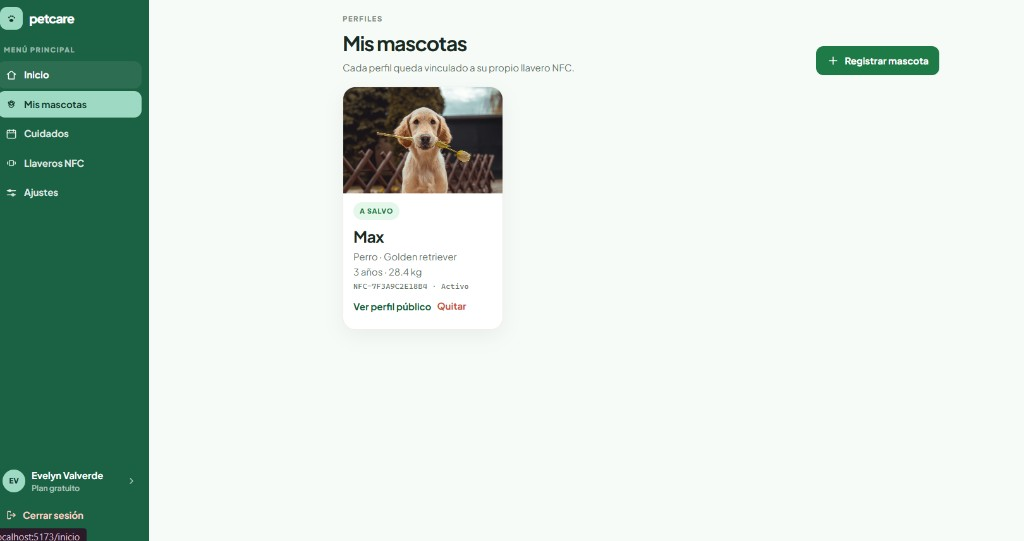
\includegraphics[width=0.78\textwidth]{04-mascotas.png}
\caption{Mis mascotas. Cada ficha muestra su llavero y el enlace a su perfil público.}
\end{figure}

\subsection{Fotos de la mascota}

En el mismo registro se pueden subir hasta tres fotos. El control muestra cuántas van de tres y avisa que la primera es la principal. Si se intenta agregar una cuarta, el formulario lo dice en el acto. Cada miniatura se puede quitar antes de guardar. Las fotos son opcionales: una ficha sin imagen usa las iniciales del nombre.

La primera foto es la que se ve en la tarjeta, en el inicio y como imagen grande del perfil público. Si hay más de una, el perfil permite cambiar cuál se muestra.

\begin{figure}[ht]
\centering
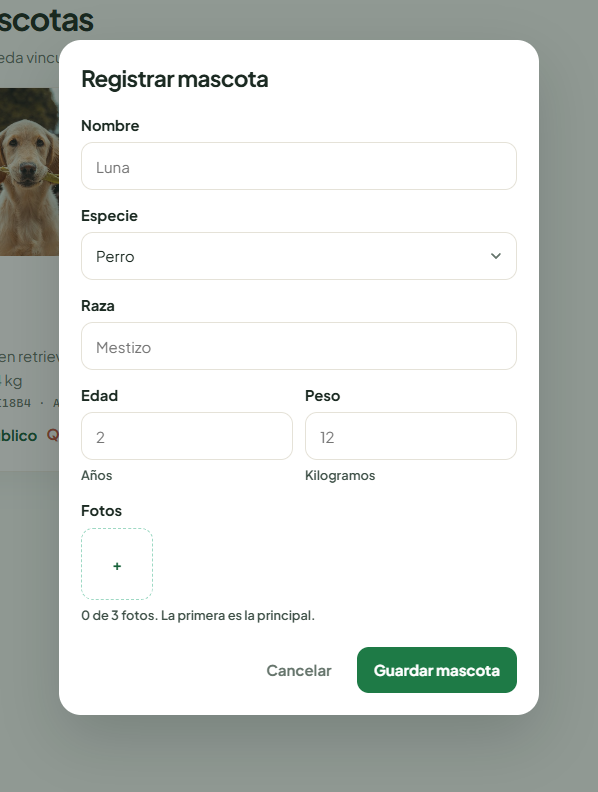
\includegraphics[width=0.62\textwidth]{05-registrar.png}
\caption{Registrar mascota. El campo de fotos admite como máximo tres imágenes.}
\end{figure}

\subsection{Cuidados}

La agenda se filtra en Todos, Vacunas, Citas y Desparasitación. Cada tarjeta dice el tipo, el título, la fecha y el lugar. En Max aparecen la vacuna antirrábica, el control veterinario y la desparasitación interna. Estas fechas no se publican en el perfil del llavero. El texto de la pantalla lo dice de entrada.

\begin{figure}[ht]
\centering
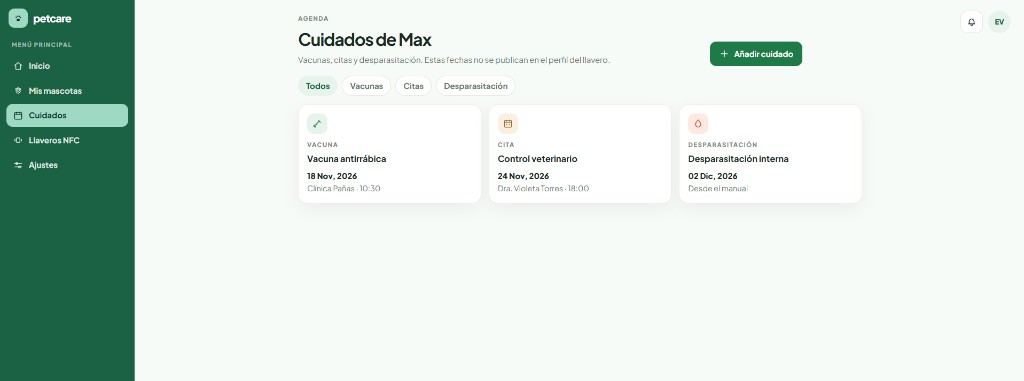
\includegraphics[width=0.92\textwidth]{06-cuidados.png}
\caption{Cuidados de Max. La agenda es privada y se puede filtrar por tipo.}
\end{figure}

\subsection{Llaveros NFC}

Cada llavero muestra a qué mascota pertenece, su código largo y si está activo. El de Max está activo, con el código \texttt{NFC-7F3A9C2E18B4}. El texto explica la consecuencia de desactivarlo: quien acerque el celular ya no verá el contacto de la dueña.

\emph{Simular escaneo del llavero} abre el perfil público, el mismo que vería alguien con el collar. No hace falta un lector NFC físico para revisar qué quedó visible. Si más adelante el mismo enlace se imprime como código QR, la pantalla de destino no cambia.

\begin{figure}[ht]
\centering
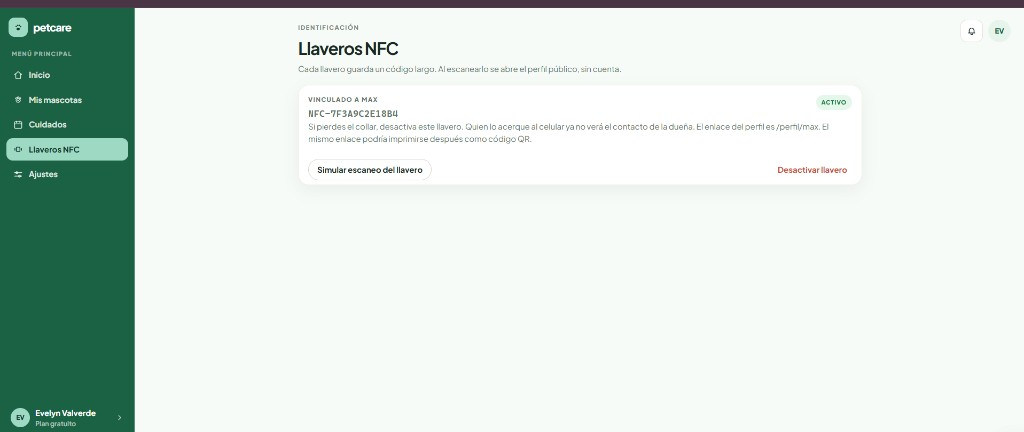
\includegraphics[width=0.92\textwidth]{07-llaveros.png}
\caption{Llaveros NFC. Desactivar el código oculta el contacto de la dueña al escanear.}
\end{figure}

\subsection{Perfil público, extravío y ajustes}

El perfil público ocupa la ventana. Arriba quedan el logo y el regreso al panel, o la entrada para la dueña si quien mira no tiene sesión. La foto va a un lado y los datos al otro: nombre, especie, raza, edad y dueña. Si la mascota está marcada como extraviada, el perfil lo dice con un aviso visible. Si el llavero se desactivó, no se muestra el celular ni el formulario.

Quien encuentra al animal puede escribir su nombre y un mensaje. Ese aviso aparece en la campana del panel de la dueña. En Ajustes, la cuenta decide dos cosas: si el celular se muestra y si el formulario de aviso sigue disponible. El nombre y el teléfono de la dueña también se actualizan ahí. La dirección no tiene un control para publicarse, porque no forma parte del perfil.

\section{Evaluación con heurísticas}

Las diez heurísticas de Nielsen sirven aquí como lista de revisión del flujo, no como una prueba con usuarios. La tabla resume dónde se aplican en las pantallas ya construidas.

\begin{table}[ht]
\centering
\small
\begin{tabularx}{\textwidth}{l X}
\toprule
\textbf{Heurística} & \textbf{Cómo se ve en PetCare} \\
\midrule
Visibilidad del estado & A salvo, Extraviado, Activo e Inactivo, y el texto Guardando al registrar. \\
Correspondencia con el mundo & Se habla de llavero, collar, cita y kilogramos, no de identificadores internos. \\
Control y libertad & Los formularios tienen Cancelar. El extravío se puede revertir. El llavero se reactiva. \\
Consistencia & El verde y el menta del acceso se repiten en el menú, los botones y las etiquetas. \\
Prevención de errores & Especie cerrada, edad de 0 a 30, peso revisado y máximo de tres fotos. \\
Reconocer antes que recordar & La cuenta de ejemplo se escribe sola. El código NFC se ve en la ficha. \\
Flexibilidad & Recordarme cambia la duración de la sesión. Varias mascotas conviven en la misma cuenta. \\
Diseño sobrio & El perfil público no muestra vacunas, citas ni dirección. \\
Recuperación ante errores & Los campos inválidos explican el problema en español, junto al dato. \\
Ayuda en contexto & El celular, el límite de fotos y el efecto de desactivar el llavero se explican en la misma pantalla. \\
\bottomrule
\end{tabularx}
\caption{Revisión del flujo con las heurísticas de Nielsen.}
\end{table}

Shneiderman pide, entre sus reglas, retroalimentación y acciones reversibles. PetCare responde al guardar una mascota con el código del llavero recién creado, y permite deshacer el extravío o volver a activar el collar. La confirmación al quitar una mascota cubre el caso que no conviene deshacer a la ligera, porque borra también el perfil que vería quien escanea.

La revisión heurística no sustituye una prueba con dueñas reales. Sirve para dejar escrito por qué cada pantalla está recortada y qué estado debe verse después de cada acción. Una siguiente evaluación podría observar a una persona que encuentra el perfil sin explicación previa y medir si localiza el celular o el formulario sin entrar al panel.

\section{Qué sostiene el recorrido}

La interfaz está hecha con React y el servidor con Node y Express, en el mismo proyecto. Al ejecutar \texttt{npm run dev} se abren los dos: la página, normalmente en \url{http://localhost:5173}, y la API en el puerto 8787. Las cuentas, las mascotas, los cuidados, los llaveros y los avisos se guardan en el servidor. Las contraseñas no se almacenan en texto plano. Una sesión nueva no comparte los datos de otra.

Esto importa para la interacción. Reportar un extravío no cambia solo la etiqueta de la pantalla actual: el perfil público, abierto en otro navegador y sin sesión, muestra el mismo estado. Desactivar el llavero oculta el contacto también para quien no está en el panel. El aviso enviado desde el perfil llega a la campana de la dueña.

El código del proyecto está publicado en \url{https://github.com/Eve050/PetCare}. La aplicación se recorre en local con la cuenta de ejemplo. No está desplegada en un hosting aparte.

\section{Conclusiones}

El flujo queda cerrado en las dos direcciones que pide el caso. La dueña entra, reconoce a Max y puede marcarlo como extraviado. Quien escanea el llavero abre un perfil sin cuenta, ve solo lo autorizado y puede dejar un aviso. Las pantallas de acceso, inicio, mascotas, cuidados y llaveros usan la misma paleta y separan lo privado de lo público.

Las decisiones de interfaz que más cuidan a la segunda persona son las menos visibles en el panel: no publicar la agenda, explicar para qué sirve el celular, limitar las fotos a tres y decir qué pasa si el llavero se desactiva. Esas frases cortas, puestas junto al control, reducen la necesidad de un manual.

El recorrido ya se puede repetir con datos guardados, no solo con una maqueta. La cuenta de ejemplo conserva a Max, la Clínica Pañas, la Dra.~Violeta Torres y el llavero \texttt{NFC-7F3A9C2E18B4}. Una cuenta nueva empieza vacía y arma su propia ficha, su código y, si la dueña lo desea, hasta tres fotos.

\begin{thebibliography}{9}
\bibitem{iso} International Organization for Standardization. (2019). \emph{ISO 9241-210:2019. Ergonomics of human-system interaction — Part 210: Human-centred design for interactive systems}.
\bibitem{krug} Krug, S. (2014). \emph{Don't make me think, revisited: A common sense approach to web usability} (3rd ed.). New Riders.
\bibitem{nielsen1994} Nielsen, J. (1994). Enhancing the explanatory power of usability heuristics. \emph{Proceedings of the SIGCHI Conference on Human Factors in Computing Systems}, 152--158.
\bibitem{nielsen2024} Nielsen, J. (2024). \emph{10 usability heuristics for user interface design}. Nielsen Norman Group. \url{https://www.nngroup.com/articles/ten-usability-heuristics/}
\bibitem{norman} Norman, D. (2013). \emph{The design of everyday things} (Revised and expanded ed.). Basic Books.
\bibitem{shneiderman} Shneiderman, B., Plaisant, C., Cohen, M., Jacobs, S., Elmqvist, N., \& Diakopoulos, N. (2016). \emph{Designing the user interface: Strategies for effective human-computer interaction} (6th ed.). Pearson.
\end{thebibliography}

\end{document}
